\documentclass[]{beamer} %aspectratio=169
\usepackage[english,russian]{babel}
\usepackage[utf8]{inputenc}
\usepackage{graphicx}
\usepackage{import}
% Стиль презентации
\usetheme{Warsaw}
\setbeamertemplate{navigation symbols}{}
\setbeamertemplate{footline}[frame number]
% \beamertemplatenavigationsymbolsempty
\graphicspath{{./img/}{./img/giftWraping2D/}{./img/firstPlane/}{./img/crossP/}{./img/crossPN/}{./img/heap/}}
\usefonttheme[onlymath]{serif}
\def\svgwidth{\linewidth}
\begin{document}
\title{МНОГОМЕРНЫЙ АЛГОРИТМ ОВЫПУКЛЕНИЯ РОЯ ТОЧЕК, НАХОДЯЩИХСЯ В НЕОБЩЕМ ПОЛОЖЕНИИ}
\author[Корабельников А.А.]{\scriptsize Выполнил: студент гр. МЕНМ-280901 Корабельников А.А.\\Научный руководитель: к.ф.-м.н., доцент Кумков С.С}
\institute{Институт естественных наук и математики}
\date{Екатеринбург, 2020}
% Создание заглавной страницы
\frame{\titlepage}
% Автоматическая генерация содержания
% \frame{\frametitle{Содержание}\tableofcontents}
\begin{frame}{Необщее положение точек}
%     Разработать алгоритм построения выпуклой оболочки многомерного роя точек, находящихся в необщем положении.
%    \vfill
   Необщее положение точек означает что в гиперплоскости евклидова пространства размерности $d$ лежит больше чем $d +1$ точка.\\
   \vfill
    \begin{minipage}{.49\textwidth}
    \centering
    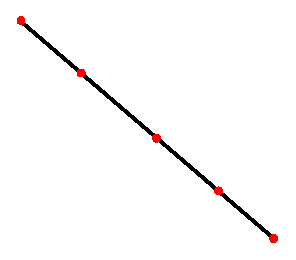
\includegraphics[width=0.5\linewidth]{line.eps}
  \end{minipage}
  \begin{minipage}{.49\textwidth}
    \centering
    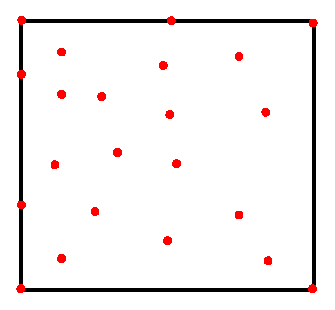
\includegraphics[width=0.5\linewidth]{cube1.eps}
  \end{minipage}
   % Пояснение в пространстве.fff
\end{frame}

\begin{frame}{Проблема необщего положения}
     \begin{minipage}{.49\textwidth}
     \centering
     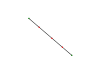
\includegraphics[width=0.8\linewidth]{line2.pdf}
   \end{minipage}
   \begin{minipage}{.49\textwidth}
     \centering
     \includegraphics[width=0.8\linewidth]{cube12.eps}
   \end{minipage}

   \bigskip

   Проблемы:
   \begin{itemize}
    \item  Требуется вычислять вершины \textbf{\textit{(гипер)грани}},
    \item  Требуется вычислять \textbf{\textit{(гипер)рёбра}} грани.
    \end{itemize}
   \vfill
   Мне не известны реализации алгоритмов овыпукления, работающих в многомерном пространстве в необщем положении.
    % В многомерном пространсве эти проблемы есть, в двухмернос одни легко решаются. Объяснить сокращение.
 \end{frame}


 \begin{frame}{Актуальность}

        \vspace{0.5cm}
        % \begin{itemize}
            % \item  Quickhull - $O(n^{\left[d/2\right]})$
            % \item  Method of Clarkson and Shor  - $O(n^{\left[d/2\right]})$

            % \medskip
            % Эти два алгоритма работают в общем положении.
            % \medskip

             Многие алгоритмы для случая плоскости имеют свои аналоги в 3D, но не в большей размерности.
        % \end{itemize}
        \vspace{0.25cm}

        Библиотеки вычислительной геометрии:
        \begin{itemize}
            \item  CGAL
            \item  LEDA
        \end{itemize}
        \vfill
        \begin{center}
            \raisebox{20mm}{
            \parbox{0.5\textwidth}{Основная проблема алгоритмов, нацеленных на общее положение --- несимплициальные грани.}
            }
            \hspace{10mm}
            \includegraphics[width=0.3\linewidth]{wrongCube.pdf}
        \end{center}
        \vfill
        % Многие алгоритмы в плоскости имеют свои аанлоги, имеются реализации вот таких библиотеках и рализованно тотлько одля общего случая.
\end{frame}

\begin{frame}{Цель работы}
    Разработать алгоритм построения выпуклой оболочки многомерного роя точек, находящихся в необщем положении.
\end{frame}

\begin{frame}{Алгоритмы овыпукления на плоскости}
    Существует множество алгоритмов овыпукления на плоскости:
    \begin{itemize}
        \item  \textbf{Gift wrapping --- $O(nh)$}
        \item  Graham scan --- $O(n \log n)$
        \item  Quickhull --- $O(n \log n)$
        \item  Divide and conquer --- $O(n \log n)$
        \item  Monotone chain --- $O(n \log n)$
        \item  Chan's algorithm --- $O(n \log n)$
    \end{itemize}
    \vfill
    Для развития был взят алгоритм заворачивания подарка, т.к. он менее всего использует специфику плоскости.
      % На плоскости много алгоритмов. Для многомерного случая он реализован в библиотеках segal b leda.
\end{frame}

\begin{frame}[t]{Алгоритм Джарвиса на плоскости}
    \vspace*{-10mm}
    \centering{
      \includegraphics<1>[width=0.7\linewidth]{gift.pdf}%
      \includegraphics<2>[width=0.7\linewidth]{gift2.pdf}%
      \includegraphics<3>[width=0.7\linewidth]{gift3.pdf}%
      \includegraphics<4>[width=0.7\linewidth]{gift4.pdf}%
      \includegraphics<5>[width=0.7\linewidth]{gift5.pdf}%
      \includegraphics<6>[width=0.7\linewidth]{gift6.pdf}%
      \includegraphics<7>[width=0.7\linewidth]{gift7.pdf}%
      \includegraphics<8>[width=0.7\linewidth]{gift7_5.pdf}%
      \includegraphics<9>[width=0.7\linewidth]{gift9.pdf}%
      \includegraphics<10>[width=0.7\linewidth]{gift10.pdf}%
      \includegraphics<11>[width=0.7\linewidth]{gift11.pdf}%
      \includegraphics<12>[width=0.7\linewidth]{gift13.pdf}%
      \includegraphics<13>[width=0.7\linewidth]{gift14.pdf}%
    }
    % \vspace*{-6mm}

    % \only<1-4>{Построение первой грани}
    \centering{
    \only<1>{Пусть есть множество точек $P=\{p_1, p_2,\ldots p_9\}$, $P \in R^2$.}%
    \only<2>{Находим минимальную точку. Проводим через нее прямую, параллельную оси $Oy$.}%
    \only<3>{Поочередно проводим векторы к свободным точкам.}%
    \only<4>{Берем точку, направление на которую образует максимальный угол с направляющим вектором выбранной прямой.}%
    \only<5>{Начальная грань построена. Находим вектор ребра.}%
    \only<6-12>{Построение следующего ребра.}%
    \only<13->{Конец построения}%
    }
\end{frame}

\begin{frame}{Этапы}
       \begin{itemize}
        \item  Разработать реализацию многомерного алгоритма Джарвиса для общего положения точек;
        \item Расширить реализацию для работы при необщем положеии точек.
        \end{itemize}
\end{frame}

% \begin{frame}{Алгорим Джарвиса при общем положении точек}
%     Проблемы расширения:
%        \begin{itemize}
%         \item  поиск первой грани;
%         \end{itemize}
% \end{frame}
% Хранение это тяжело, но если у нас симликтически грани,
% \begin{frame}{Хранение выпуклой оболочки}
%     Грань -  Симплекс.
%     \vfill
%     Граф $G:=(V,E)$ , где $V$- непустое множество граней выпуклой оболочки, а $E$ — множество пар соседних граней.
% \end{frame}


    % Базис всех кординатных осей, кроме Ox1;
% Выкинули первый вектор базиса и начали добавлять из текущей точки в пробную точку, находя нормаль.
%Продолжая с остальными веркторами базса туже самую процедуру.
% Далее не доделано, остальное будет доделан в следю раз

\begin{frame}[t]{Поиск первой грани}
    \vspace*{-8mm}\hspace*{15mm}%
        \only<1>{\noindent\input{./img/firstPlane/first.pdf_tex}}%
        \only<1>{\input{./img/firstPlane/first1.pdf_tex}}%
        \only<2>{\input{./img/firstPlane/first2.pdf_tex}}%
        \only<3>{\input{./img/firstPlane/first3.pdf_tex}}%
        \only<4>{\input{./img/firstPlane/first3_1.pdf_tex}}%
        \only<5>{\input{./img/firstPlane/first4.pdf_tex}}%
        \only<6>{\input{./img/firstPlane/first5.pdf_tex}}%
        \only<7>{\input{./img/firstPlane/first6.pdf_tex}}%
        \only<8>{\input{./img/firstPlane/first6_1.pdf_tex}}%
        \only<9>{\input{./img/firstPlane/first7.pdf_tex}}%
        \only<10>{\input{./img/firstPlane/first8.pdf_tex}}%
        \only<11>{\input{./img/firstPlane/first9.pdf_tex}}%
    \centering{
    \only<1>{ \par Находим минимальную точку и проводим через нее плоскость, перпендикулярной первой кординатной оси.}
    \only<2>{\vspace*{-3mm}\par Формируем базис плоскости из векторов базиса пространства. \\ Создаем базис подпространства, исключая первый вектор базиса плоскости.}%
    \only<3>{\par Поочередно проводим векторы к свободным точкам. }%
    \only<4>{Ортонормируем эти векторы на фоне базиса подпространства\\ (шаг процедуры Грама–Шмидта)}
    \only<5>{\vspace*{-5mm}\par  Выбираем вектор, образующий наибольший угол с исключенным вектором базиса. Запоминаем точку. Заменяем исключенный вектор базиса. }%
    \only<6>{\par Создаем базис подпространства, исключая второй вектор базиса плоскости.}%
    \only<7>{\par Поочередно проводим векторы к свободным точкам. }%
    \only<8>{Ортонормируем эти векторы на фоне базиса подпространства\\ (шаг процедуры Грама–Шмидта)}
    \only<9>{\vspace*{-5mm}\par Выбираем вектор, образующий наибольший угол с исключенным вектором базиса. Запоминаем точку. Заменяем исключенный вектор базиса. }%
    \only<10>{После нужного количества повторений этой операции получаем плоскость начальной грани. }
    \only<11>{\par Начальная грань найдена. Грань добавляется в очередь на рассмотрение. }%
    % \only<4>{\par Базис новой плоскости формируется из базиса ребра и вектора в точку.}%

    }
\end{frame}
% \begin{frame}{Алгорим Джарвиса при общем положении точек}
%     Проблемы расширения:
%        \begin{itemize}
%         \item  поиск первой грани;
%         \item  обход граней.
%         \end{itemize}
% \end{frame}

\begin{frame}{Обход граней}
    \begin{itemize}
        \item Процесс перебора и создания граней допускает графовую формализацию. Поиск в ширину.
        % \item Перебор ребер очередной грани и переход на соответствующую соседнюю грань   --- обход в ширину.
        \item Хранение информации о найденных гранях --- хеш-таблица.
        \item Хеш вычисляется на основе целых чисел, получаемых из коэффициентов уравнения плоскости грани.
        % Возможны и другие алгоритмы хэширования граней: на основе точек вершин, на основе индексов точек вершин.
    \end{itemize}
    \vfill
    \pause
    Порядок обхода
    \begin{itemize}
        \item берем необработанную грань;
        \item для каждого ребра выполняем переход на соседнюю грань;
        \item если найденная грань еще не обрабатывалась, добавляем в очередь.
    \end{itemize}
\end{frame}

\begin{frame}[t]{Как происходит переход через ребро }
    \vspace*{-8mm}\hspace*{15mm}%
    \only<1>{\input{./img/crossP/cross.pdf_tex}}%
    \only<2>{\input{./img/crossP/cross_01.pdf_tex}}%
    \only<3>{\input{./img/crossP/cross_02.pdf_tex}}%
    %\only<4>{\input{./img/crossP/cross_03.pdf_tex}}%
    \only<4>{\input{./img/crossP/cross_05.pdf_tex}}%
    \only<5>{\input{./img/crossP/cross1.pdf_tex}}%
    \only<6>{\input{./img/crossP/cross2.pdf_tex}}%
    \only<7>{\input{./img/crossP/cross3.pdf_tex}}%

    % \vspace*{-3mm}
    % Если очередь граней на обработку не пуста забираем грань из очереди.
    % и рассматриваем его.
\centering{
    \only<1>{Берем очередное ребро грани и поворачиваем вокруг него плоскость грани. }
    \only<2>{Находим базис ребра.}
    \only<3>{Проводим вектор к свободной точки грани и ортонормируем этот вектор на фоне базиса ребра. \\ (шаг процедуры Грама–Шмидта)}
    \only<4>{Поочередно проводим вектора к свободным точкам грани.}
    \only<5>{Ортонормируем эти векторы на фоне базиса ребра.}
    \only<6>{Берем плоскость, образующую максимальный угол с предыдущей гранью.}
    \only<7>{Грань найдена. Если грань новая, то добавляем ее в очередь на обработку.  Переходим к рассмотрению следующего ребра предыдущей грани.}
}
\end{frame}


\begin{frame}{Результат}

    % Для обхога всех граней был использован обход в ширину.
    % При обработки грани, для всех ее ребер находятся соседние грани.
    % Если грань новая то ее добавляют в очередь
    % Для хранения информации о найденных гранях была использована хэш таблица.
    Сложность --- $O(n\cdot F\cdot d^2)$,\\
    где $F$ --- количество граней, $n$ --- количество точек, $d^2$~---~порядок количества ребер у $d$-мерного симплекса.
    % \vfill
    % \begin{center}
    %     \includegraphics[width=0.6\linewidth]{simplex.jpg}%
    % \end{center}

    \medskip

    Операция перехода через ребро выполняется $d^2$ раз для каждой из $F$ граней выпуклой оболочки. При этом перебираются почти все точки роя, которых $n$ штук.
    % Если для расматриваемого ребра была уже найдена
    %
    % Хэш при неточных вычислениях.
    % Описать метод хеширования.
    % Перебор точек.
\end{frame}
\begin{frame}{Алгорим Джарвиса при необщем положении точек}
 % Грань -  Симплекс.ував
    % \vfill
    Проблемы расширения на случай необщего положения точек:
       \begin{itemize}
        \item  построение грани;
        \end{itemize}
\end{frame}


% \begin{frame}{Хранение выпуклой оболочки}


%     % При $R^n$ $\left(n>2\right)$ грань $v$ --- выпуклая оболочка, граф $F'\in R^{n-1}$.

%     % При $R^2$ грань $v$ --- массив точек $P$.
% \end{frame}


\begin{frame}{Проблема построения грани}

    Проблемы построения:
    \begin{itemize}
        \item  априори невозможно указать, какие из точек, попавших в плоскость грани, являются ее вершинами;
        \item грани выпуклой оболочки могут содержать разное количество ребер.
    \end{itemize}
    % В плоскости грани могут содержаться точки, не являющиеся вершинами этой грани.
    \pause

    Решение --- уход в аффинное подпространство плоскости грани и построение в нем выпуклой оболочки роя точек, попавших в эту плоскость.

    Отдельное рассмотрение случая двумерного аффинного подпространства.

    \hspace*{10mm}
    \begin{minipage}{.3\textwidth}
        \centering
        \includegraphics[width=\linewidth]{affine.pdf}
      \end{minipage}
      \begin{minipage}{.1\textwidth}
        \centering
        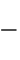
\includegraphics[width=0.8\linewidth]{affine2.pdf}
      \end{minipage}
      \begin{minipage}{.3\textwidth}
        \centering
        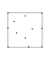
\includegraphics[width=\linewidth]{affine1.pdf}
      \end{minipage}

    % \vfill
    % \begin{center}
    %     \includegraphics[scale = 0.5]{./images/square.png}
    % \end{center}

\end{frame}
% Эти проблемы решаются уходом в афинное подпространстов грани. И построением выпуклой оболочки там.
% ДЛя этого нужно расширить алгоритм общего положения.
% После того как плоскость грани найдена, решая недоопределенную систему линейных уравлений находим нормаль плоскости.
% С помощью нормали находим все точки и переводим их координаты в базис плоскости.
%После этого ищем выпуклую оболочку набора точек.
\begin{frame}[t]{Поиск первой грани}
    \vspace*{-8mm}\hspace*{15mm}%
    \only<1>{\input{./img/affinePoint.pdf_tex}}%
    \only<2>{\input{./img/affinePoint05.pdf_tex}}%
    \only<3>{\input{./img/affinePoint1.pdf_tex}}%
    \only<4>{\input{./img/affinePoint15.pdf_tex}}%
    \only<5>{\input{./img/affinePoint16.pdf_tex}}%
    \only<6>{\input{./img/affinePoint3.pdf_tex}}%


\centering{
    \only<1>{Находими плоскость грани. После этого в сравнении с предыдущим алгоритмом производятся дополнительные шаги. \\}%
    \only<2>{Вычисляем нормаль плоскости \\}%
    \only<3>{Находим точки и пересчитываем их в базис плоскости \\}%
    \only<4>{Строим выпуклую оболочку \\}%
    \only<5>{Если базисы ребер неизвестны, находим. Запоминаем базисы. \\}%
    \only<6>{\vspace*{-3mm}Заменяем точки выпуклой оболочки на исходные и пересчитываем базисные векторы ребер в координаты исходного пространства. Добавляем грань в очередь на обработку. \\}%
}
\end{frame}

\begin{frame}{Алгорим Джарвиса при необщем положении точек}
    % Грань -  Симплекс.ував
       % \vfill
       Проблемы расширения:
          \begin{itemize}
            \item  построение грани;
           \item  хранение выпуклой оболочки;
           \end{itemize}
\end{frame}

\begin{frame}{Хранение выпуклой оболочки}
    % В результате появляются новые требования к хранению.

    % \begin{itemize}
    %     \item в несимплициальном случае недостаточно хранить только вершины, нужно хранить ребра, которые в свою очередь могут быть многомерными несимплициальными многогранниками;
    %     \item для дальнейшего использования разумно хранить список и информацию о плоскости грани соседних граней;
    % \end{itemize}
    Необходимо хранить:
    \begin{itemize}
        \item Информацию о ребрах: список ребер и их базисы.
        \item необходимо хранить список соседних граней;
        \item нужно хранить информацию о плоскости грани:
        \begin{itemize}
            \item аффинный базис: линейный базис и опорную точку;
            \item уравнение плоскости;
        \end{itemize}
    \end{itemize}

    % \pause
    % \vfill

    % % Решение:

    % % Выпуклая оболочка $n$ - мерного пространства, это граф $F:=(V,E)$ , где $V$- непустое множество граней, а $E$ - множество пар соседних граней.

    % Грань хранит:
    % \begin{itemize}
    %     \item информацию плоскости:
    %     \item список соседних граней;
    %     \item структура грани:
    %     \end{itemize}

    %Для дальнейших вычислений необходимо хранить базис и уравнения плоскости. для каждой грани.
\end{frame}



\begin{frame}{Алгорим Джарвиса при необщем положении точек}
    % Грань -  Симплекс.ував
       % \vfill
       Проблемы расширения:
          \begin{itemize}
            \item  построение грани;
           \item  хранение выпуклой оболочки;
           \item  обход ребер.
           \end{itemize}

           Переход через ребро осуществляется точно так же, как и в случае общего положения точек. После нахождения плоскости грани, возможен рекурсивный вызов алгоритма.
\end{frame}

% \begin{frame}[t]{Переход через ребро}
%     \vspace*{-8mm}\hspace*{15mm}%
%     \only<1>{\input{./img/crossPN/crossPN1.pdf_tex}}%
%     \only<2>{\input{./img/crossPN/crossPN2.pdf_tex}}%
%     \only<3>{\input{./img/crossPN/crossPN3.pdf_tex}}%
%     \only<4>{\input{./img/crossPN/crossPN4.pdf_tex}}%
%     \only<5>{\input{./img/crossPN/crossPN5.pdf_tex}}%
%     % \only<6>{\input{./img/crossPN/crossPN6.pdf_tex}}%
%     \only<6-7>{\input{./img/crossPN/crossPN7.pdf_tex}}%
%     \only<8-9>{\input{./img/crossPN/crossPN8.pdf_tex}}%
%     \only<10>{\input{./img/crossPN/crossPN9.pdf_tex}}%

%     % \vspace*{-3mm}
% \centering{
%     % Если очередь граней на обработку пуста, остановить работу
%     \only<1>{Пока очередь граней на обработку не пуста повторять.\\ Взять грань из очереди. \\}%
%     \only<2>{Взять очередное ребро обрабатываемой грани.\\}%
%     \only<3>{Поочередно провести векторы к свободным точкам.\\}%
%     \only<3>{Ортонормировать эти векторы на фоне базиса ребра \\(шаг процедуры Грама--Шмидта) \\}%
%     \only<4>{Найти вектор, образующий максимальный угол с вектором грани. \\}%
%     \only<5>{Плоскость грани найдена.\\}%
%     \only<6>{ Определить нормаль плоскости. Построить хэш плоскости грани и проверить, обработана ли она уже. \\ }%
%     \only<7>{Если обработана, запомнить информацию о соседстве граней и перейти к следующему ребру обрабатываемой грани. Иначе продолжить обработку новой грани. \\}
%     \only<8>{Найти точки, попавшие в плоскость грани. \\}%
%     \only<9>{Если их $d+1$ штука, то грань симплициальная и не требует особой обработки. Иначе запустить рекурсивно алгоритм овыпукления в аффинном подпространстве.\\}
%     %  и выразить их в координатах пространства плоскости грани.
%     \only<10>{Грань построена. Запомнить информацию о соседстве. Добавить в очередь на обработку.\\}%
% }
% \end{frame}
% \begin{frame}{Проблема построения грани}
%     % Как мы вытаскиваем объект исходного пространства.
%     % для этого необходимо доработать реализацию алгоритма построения выпуклой оболочки при общем положении.
%     % Напоследнем этапе постения у нас имеется базис плоскости, но нам еще известно сколько точек лежит на этой плоскости.
%     Порядок построения:
%     \begin{itemize}
%         \item найти плоскости грани;
%         \begin{itemize}
%             \item плоскость определяется нахождением симплицированной грани
%         \end{itemize}
%         \item найти уравнение плоскости;
%         \item определить точки, лежащие на плоскости;
%         \item перевести точки в базис плоскости;
%         \item найти выпуклую оболочку в координатах плоскости;
%         \item подменить точки выпуклой оболочки на исходные.
%     \end{itemize}

% \end{frame}


% \begin{frame}{Обход граней}
%     Обход происходит также как и в 2d
%     Порядок построения:
%     \begin{itemize}
%         \item поиск плоскости грани;
%         \item определение точек, лежащих на плоскости;
%         \item перевод точек в базис плоскости;
%         \item построение выпуклой оболочки в подпространстве;
%         \item подмена точек выпуклой оболочки на исходные.
%     \end{itemize}

% \end{frame}

% \begin{frame}{Алгоритм при необщем положении точек}

%     Вход --- Набор точек $R^d$ пространства;

%     Выход --- Выпуклая оболочка;
%     \begin{itemize}
%         \item Если $n = 2$ найти выпуклую оболочку на плоскости;
%         \item Если количество точек равно $n+1$ построить симплекс;
%         \item Найти первую грань и добавить ее в очередь;
%         \item Пока очередь не пуста, брать грань и производить переход для каждого ребра.
%         \item Если грань новая добавляются в очередь, иначе добавить в соседние.
%     \end{itemize}

% \end{frame}


% \begin{frame}{Поиск первой грани}

%     \begin{itemize}
%         \item Найти первую грань:
%         \begin{itemize}
%             \item найти плоскость начальной грани;
%             \item найти точки и перевести их в базис плоскости;
%             \item рекурсивно найти выпуклую оболочку;
%         \end{itemize}
%         \item добавить грань в очередь на рассмотрение;
%     \end{itemize}

% \end{frame}

% \begin{frame}{Построение выпуклой оболочки}

%     Повторять пока очередь не пустая:
%         \begin{itemize}
%         \item взять из очереди грань;
%         \item для каждого ребра грани повторить:
%         \begin{itemize}
%             \item найти плоскость соседней грани;
%             \item найти точки и перевести их в базис плоскости;
%             \item рекурсивно найти выпуклую оболочку;
%             \item если грань не обрабатывалась, добавить ее в очередь;
%             \item иначе обозначить соседство граней;
%         \end{itemize}
%     \end{itemize}

% \end{frame}


%
%

\begin{frame}{Сложность полученного алгоритма}

    % Для обхога всех граней был использован обход в ширину.
    % При обработки грани, для всех ее ребер находятся соседние грани.
    % Если грань новая то ее добавляют в очередь
    % Для хранения информации о найденных гранях была использована хэш таблица.
    Сложность --- $O\big((F\cdot n\cdot h)^{d-1}\big)$,\\
    где $F$ --- количество граней, $n$ --- количество точек, $h$ --- количество ребер у грани, $d$~---~размерность пространства.
    % \vfill
    % \begin{center}
    %     \includegraphics[width=0.6\linewidth]{simplex.jpg}%
    % \end{center}


    % Если для расматриваемого ребра была уже найдена
    %
    % Хэш при неточных вычислениях.
    % Описать метод хеширования.
    % Перебор точек.
\end{frame}


\begin{frame}{Тестовая реализация}
        \begin{itemize}
                \item Платформа -.Net Core.
                \item Язык - C\#.
        \end{itemize}
        \vfill
        \centering{
        \begin{minipage}{.3\textwidth}
            \centering
            \includegraphics[width=0.8\linewidth]{dotnet.pdf}
          \end{minipage}
          \begin{minipage}{.3\textwidth}
            \centering
            \includegraphics[width=0.8\linewidth]{csharp.pdf}
          \end{minipage}
        }
\end{frame}


\begin{frame}{Результаты тестов}
    Были проведены замеры времени исполнения:
    \begin{itemize}
        \item 3-мерный тетраэдер c общем положением точек --- 0ms (3770 ticks);
        \item 3-мерный тетраэдер с необщем положением точек (+100 точек)--- 5ms;
        \item 4-мерный симплекс с общем положением точек --- 1ms ;
        \item 4-мерный симплекс с необщем положением точек (+100 точек)--38 ms ;
        \item 3-мерный куб с лишними точками  (+100 точек)--- 6ms;
        \item 4-мерный куб с лишними точками  (+100 точек)--- 46ms.
    \end{itemize}
\end{frame}

\begin{frame}{Заключение}

    В результате работы была разработана реализация алгоритма Джарвиса  для многомерного роя точек, находящихся в необщем положении.

    \smallskip

    В дальнейшем возможна оптимизация как самого алгоритма, так и его реализации.
\end{frame}

\begin{frame}
    \centering{
    Спасибо за внимание!}
\end{frame}

\begin{frame}{Список литературы}
    \begin{thebibliography}{9}
        \bibitem{bib:preparata:eng} Preparata F. P., Shamos M. I. Computational Geometry. An Introduction.~--- New York: Springer, 1985.~--- 400~с.

        \bibitem{bib:preparata} Препарата Ф., Шеймос М. Вычислительная геометрия: Введение. пер. с англ. под ред. Банковского Ю. М.~--- М.: Мир, 1989. --- 478~с.

        \bibitem{bib:deBerg} de Berg M., Cheong O., van Kreveld M., Overmars M. Computational Geometry. Algorithms and Applications, 3rd Ed. ~--- Berlin: Springer-Verlag, 2008.~--- 398~с.
        \end{thebibliography}
\end{frame}

\begin{frame}{Список литературы}
    \begin{thebibliography}{9}
        \bibitem{bib:Ivanov} Ивановский С. А., Преображенский А. С., Симончик С. К. Алгоритмы вычислительной геометрии. Выпуклые оболочки в трехмерном пространстве // Компьютерные инструменты в образовани.~--- 2007.~--- №\,3.~--- С.~3--17.

        \bibitem{bib:kokichi} Kokichi S. Robust gift wrapping for the three-dimensional convex hull // Journal of Computer and System Sciences.~--- 1994.~--- Vol.~49, issue~2, pp.~391--407.

        \bibitem{bib:Bekl} Беклемишев Д. В. Курс аналитической геометрии и линейной алгебры.~--- М.: Наука, 2005.~--- 308~с.
        \end{thebibliography}
\end{frame}
% \begin{frame}{Пример работы алгоритма}
%     Массив точек четырехмерном пространства.
% \end{frame}
% \begin{frame}{Пример работы алгоритма}
%     Проекции граней.
%     \begin{center}
%         \includegraphics[width=0.5\linewidth]{./images/regular.jpg}
%     \end{center}
% \end{frame}


\end{document}
